\section{Publishing: KITOpen and OEP}

\begin{frame}{Day 2 - Part 6: Publishing Your Metadata}{12:15 - 13:00}
    \begin{block}{Module 6 Goal}
        The final step! Making your data public, findable, and accessible using our key platforms: \textbf{KITOpen} and the \textbf{Open Energy Platform (OEP)}.
    \end{block}
    \begin{center}
        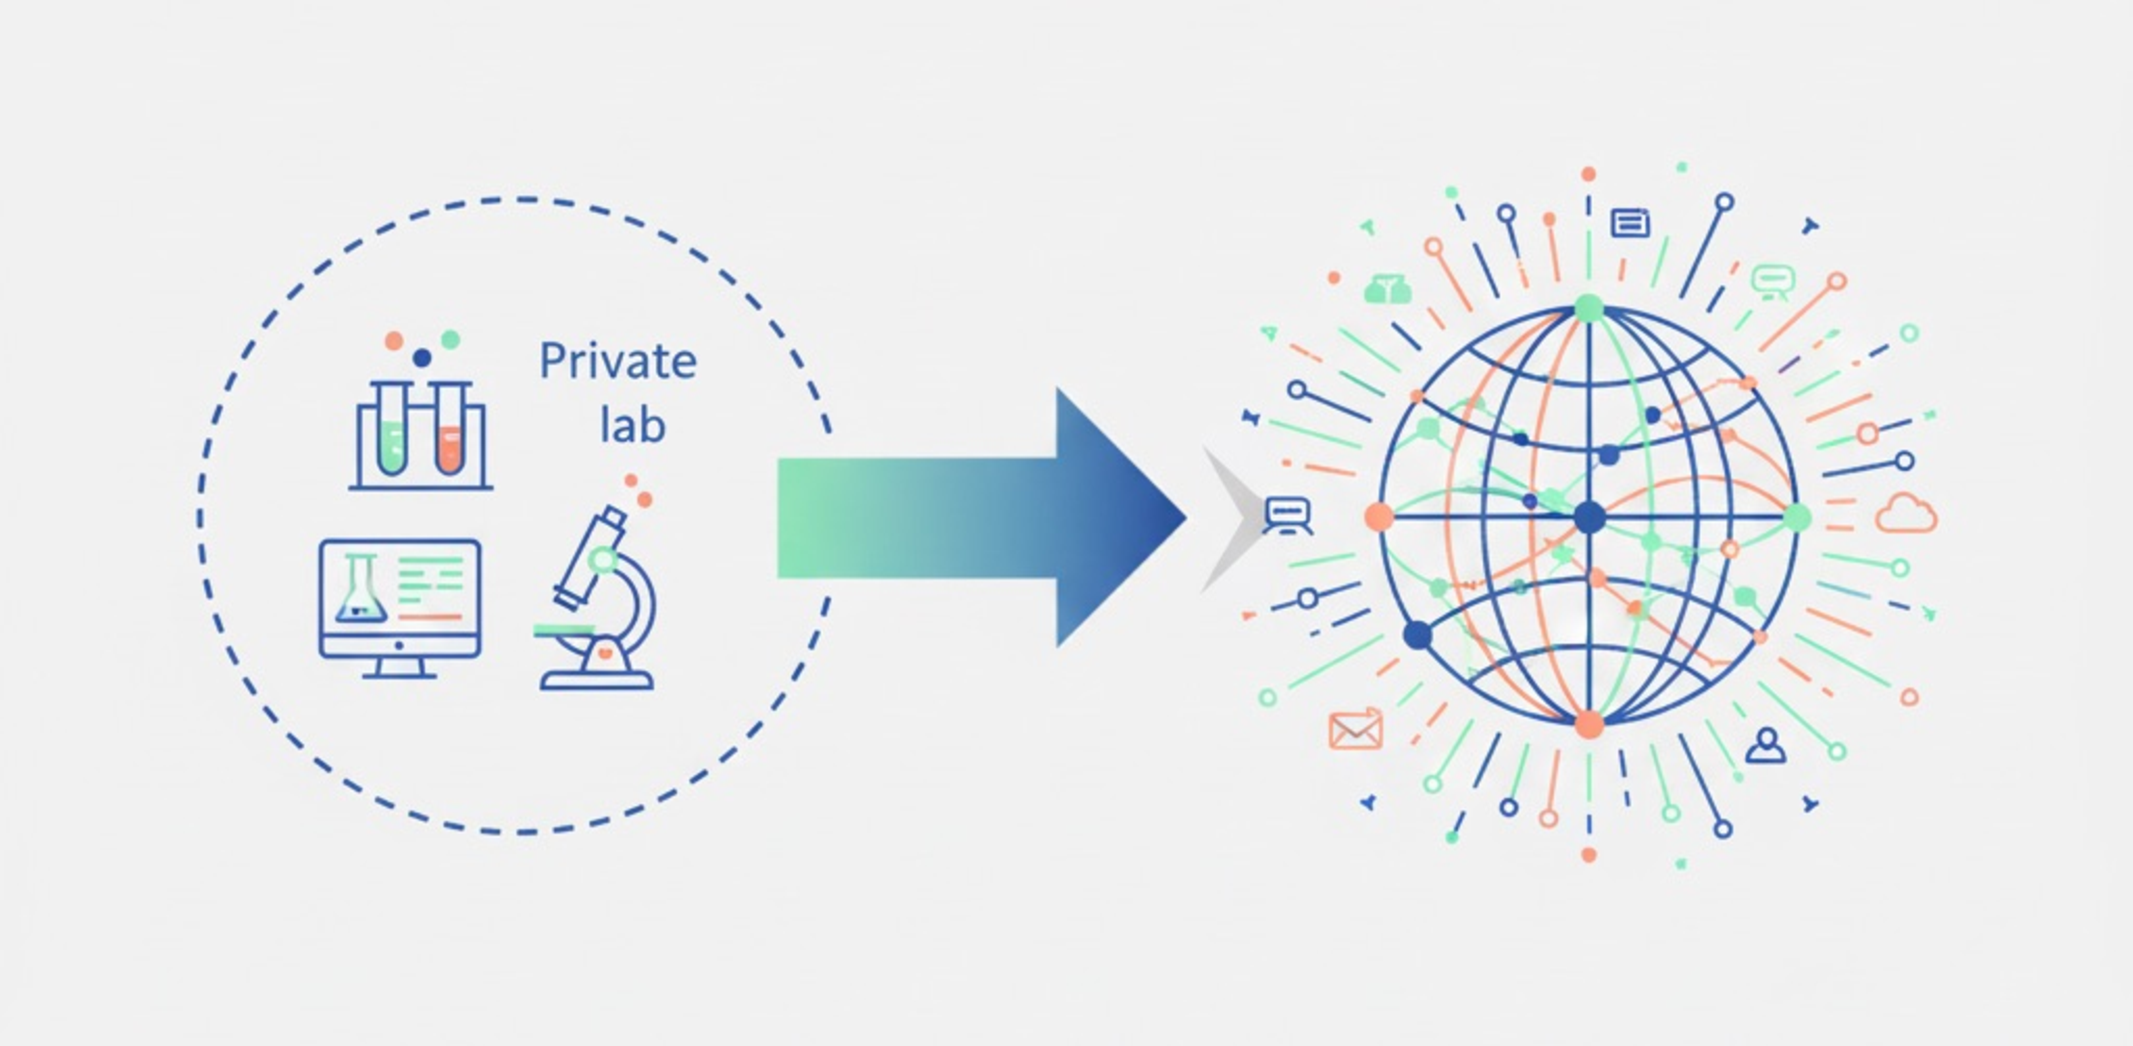
\includegraphics[width=0.36\textwidth]{figs/fig_d2p6/fig_d2p6_01-public}
        \captionof{figure}{From your lab (private) to the world (public).}
    \end{center}
\end{frame}

\begin{frame}{Learning Objectives (6.1)}
    \begin{itemize}
        \item \textbf{Identify} the mandatory submission fields for \textbf{KITOpen}.
        \item \textbf{List} the specific \textbf{domain-relevant metadata properties} unique to the \textbf{Open Energy Platform (OEP)}.
    \end{itemize}
\end{frame}

\begin{frame}{Theory: Institutional vs. Domain Repositories}{Module 6.1: Identify/List}
    \begin{columns}
        \column{.5\textwidth}
        \begin{block}{KITOpen (Institutional)}
            \textbf{Role:} Archives \emph{all} research output from KIT (papers, data, theses). \\
            \pause
            \textbf{Metadata:} General-purpose (Dublin Core). \\
            \pause
            \textbf{Mandatory Fields:}
            \begin{itemize}
                \item Title
                \item Creator (with KIT affiliation)
                \item Publication Year
                \item Resource Type (e.g., "Dataset")
                \item License
            \end{itemize}
        \end{block}
        
        \column{.5\textwidth}
        \begin{block}{Open Energy Platform (Domain)}
            \textbf{Role:} Archives \emph{only} energy research data, from \emph{all} institutions. \\
            \pause
            \textbf{Metadata:} Domain-specific. \\
            \pause
            \textbf{Domain-Relevant Properties:}
            \begin{itemize}
                \item `energy\_carrier\_type`
                \item `technology\_type`
                \item `geographic\_region (NUTS-3)`
                \item `temporal\_resolution`
            \end{itemize}
            \vspace{3.2ex}
        \end{block}
    \end{columns}
\end{frame}

\begin{frame}{Interactive: Repository Scavenger Hunt}{Module 6.1: Practice}
    \begin{block}{Activity (10 min)}
        \textbf{Task:} Open the websites for `KITOpen` and `OEP`.
        \pause
        \begin{itemize}
            \item Find the "Upload" or "Submit" page for new data.
            \item \textbf{Identify} 3 mandatory fields in KITOpen.
            \item \textbf{List} 3 \emph{domain-specific} fields in OEP that KITOpen does not have.
        \end{itemize}
        \pause
        \textbf{Discussion:} Why does OEP ask for `temporal\_resolution` while KITOpen doesn't?
    \end{block}
\end{frame}

\begin{frame}{Learning Objectives (6.2)}
    \begin{itemize}
        \item \textbf{Summarise} the process by which \textbf{KITOpen} assigns a PID (DOI) and fulfils 'F'.
        \item \textbf{Illustrate} how the community standards enforced by \textbf{OEP} enhance 'I'.
    \end{itemize}
\end{frame}

\begin{frame}{Theory: KITOpen and 'Findable'}{Module 6.2: Summarise}
    
    \begin{columns}
        \column{.36\textwidth} 
        \begin{center}
            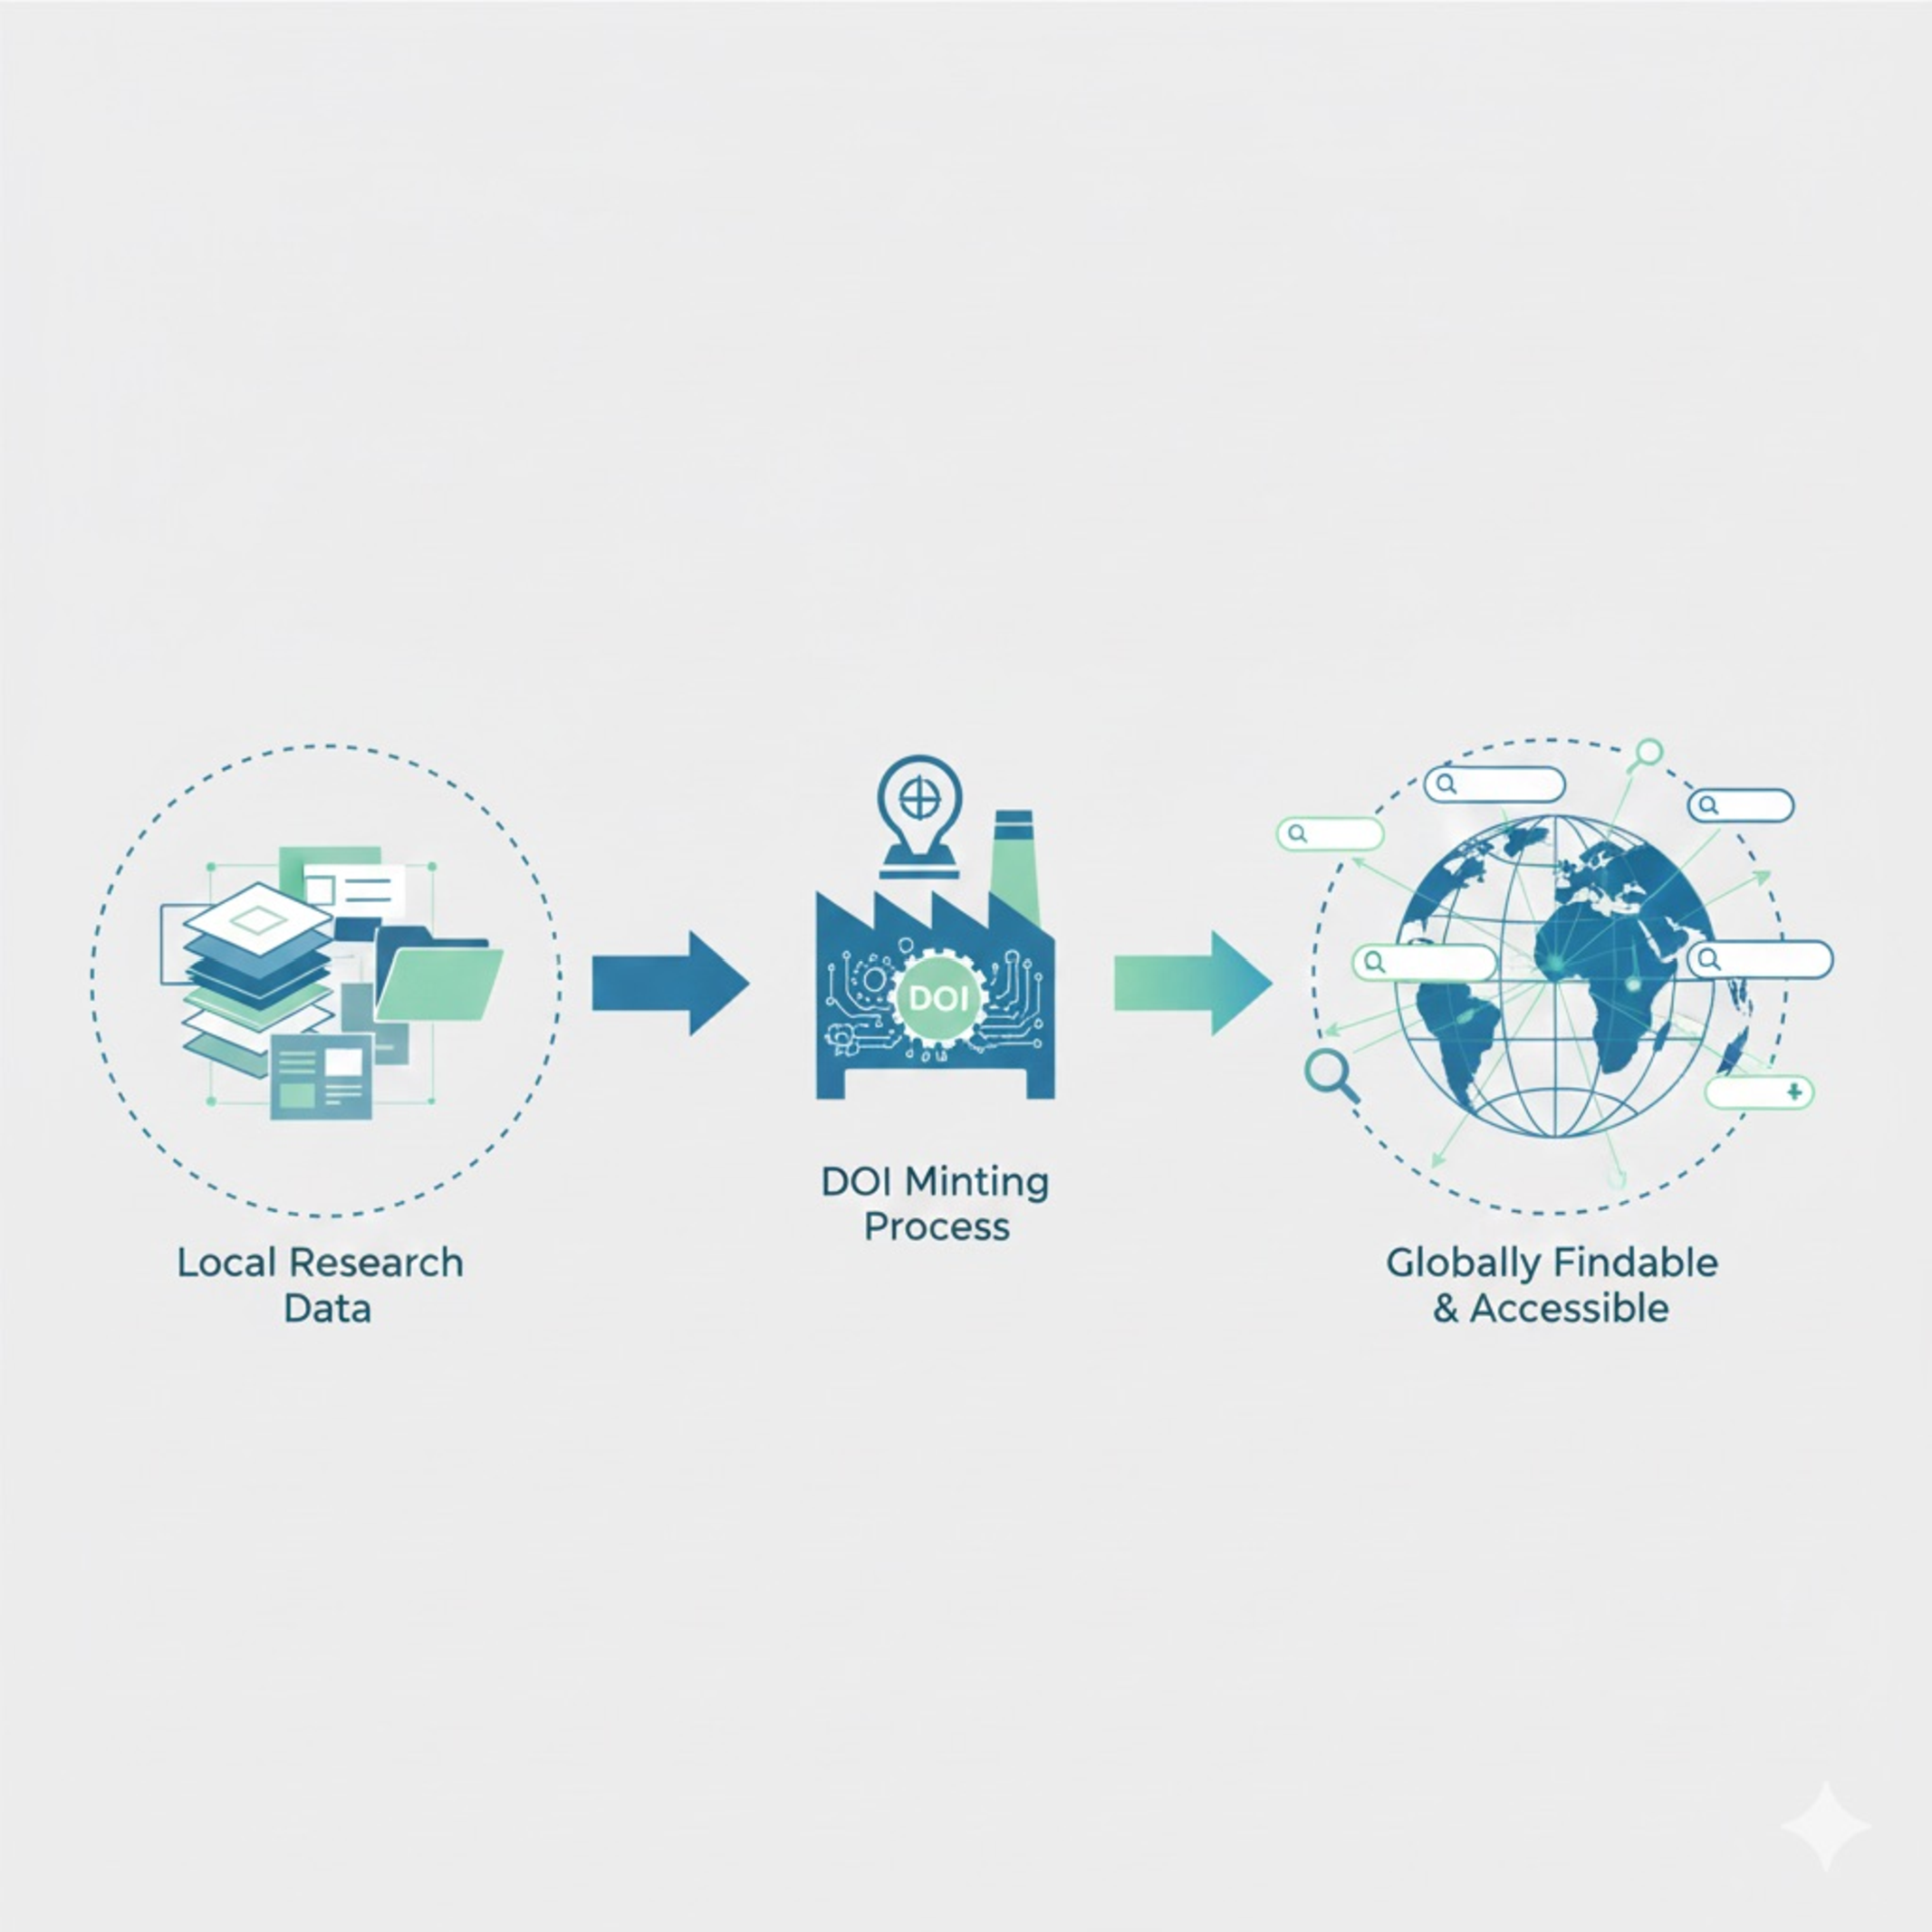
\includegraphics[width=.8\textwidth]{figs/fig_d2p6/fig_d2p6_02-mint}
            \captionof{figure}{The DOI Minting Process}
        \end{center}
        \column{.74\textwidth}
        \begin{enumerate}
            \item You upload your data to KITOpen.
            \pause
            \item You fill in the metadata (Title, Creator, etc.).
            \pause
            \item You click "Publish."
            \pause
            \item KITOpen (as a DataCite member) sends your metadata to the DOI registration agency.
            \pause
            \item A new, unique \textbf{DOI} (e.g., `10.5445/IR/100...`) is created and permanently linked to your data's metadata page on KITOpen.
        \end{enumerate}
    \end{columns}

    \pause
    Your data is now globally \textbf{Findable}.
\end{frame}

\begin{frame}{Theory: OEP and 'Interoperable'}{Module 6.2: Illustrate}
    The OEP's community standards (its metadata schema) are its power.
    
    \begin{block}{How OEP Enhances 'I'}
        \textbf{Problem:}
        \begin{itemize}
            \item You have a dataset of German power grids.
            \item A researcher from France has a dataset of French power grids.
        \end{itemize}
        \pause
        \textbf{Solution:}
        \begin{itemize}
            \item The OEP \emph{forces} both of you to use the \emph{same metadata fields} (e.g., `energy\_carrier\_type`) and the \emph{same vocabularies}.
            \pause
            \item \textbf{Result:} A third person can now write \emph{one script} to query and automatically combine both your dataset and the French dataset.
        \end{itemize}
    \end{block}
    This is \textbf{Interoperability} in action, enforced by a domain repository.
\end{frame}

\begin{frame}{Interactive: The Role of Each Repo}{Module 6.2: Practice}
    \begin{block}{Discussion (10 min)}
        \textbf{Task:}
        \begin{itemize}
            \item \textbf{Summarise:} Why is getting a DOI from KITOpen better than just putting data on your lab website?
            \pause
            \item \textbf{Illustrate:} Draw a simple diagram showing how the OEP's common standard allows two different datasets (A and B) to be combined by a third party (C).
        \end{itemize}
    \end{block}
\end{frame}

\begin{frame}{Learning Objectives (6.3)}
    \begin{itemize}
        \item \textbf{Upload} a dataset and metadata file to \textbf{KITOpen}.
        \item \textbf{Populate} an \textbf{OEP} metadata template using controlled vocabularies.
    \end{itemize}
\end{frame}

\begin{frame}{Interactive: Mock Submission (KITOpen)}{Module 6.3: Practice}
    \begin{block}{Workshop (10 min)}
        \textbf{Task:} (Conceptual or Live Demo)
        \pause
        \begin{enumerate}
            \item Take the `metadata.json` file you created in Module 4.
            \pause
            \item Go to the KITOpen submission form.
            \pause
            \item \textbf{Upload} your (dummy) data file.
            \pause
            \item Manually copy the fields (Title, Creator, etc.) from your JSON file into the corresponding fields in the KITOpen web form.
        \end{enumerate}
        \pause
        \textbf{Goal:} \textbf{Upload} (conceptually) a dataset and populate the metadata.
    \end{block}
\end{frame}

\begin{frame}{Interactive: Mock Submission (OEP)}{Module 6.3: Practice}
    \begin{block}{Workshop (10 min)}
        \textbf{Task:} Go to the OEP submission template.
        \pause
        \textbf{Challenge:} Find the field for "Geographic Region."
        \pause
        \begin{itemize}
            \item It likely requires a \textbf{controlled vocabulary} (e.g., NUTS codes).
            \item You can't just type "Karlsruhe."
            \item \textbf{Find the NUTS code for Karlsruhe.} (It's `DE122`).
        \end{itemize}
        \pause
        \textbf{Goal:} \textbf{Populate} an OEP template using a required CV.
    \end{block}
\end{frame}

\begin{frame}{Learning Objectives (6.4)}
    \begin{itemize}
        \item \textbf{Differentiate} between the institutional schema (KITOpen) and a general schema (Dublin Core).
        \item \textbf{Compare} the required access policy settings between KITOpen and OEP.
    \end{itemize}
\end{frame}

\begin{frame}{Theory: Schema Mapping (DC vs. KITOpen)}{Module 6.4: Differentiate}
    \begin{itemize}
        \item \textbf{Dublin Core (DC):} Is general. It has 15 fields.
        \pause
        \item \textbf{KITOpen Schema:} Is specific. It \textit{includes} all of Dublin Core (this is called "DC-compliance"), but adds \textbf{institutional} fields.
        \pause
        \item \textbf{Analysis:}
        \begin{itemize}
            \item `DC:Creator` $\rightarrow$ `KITOpen:Creator` (Direct map)
            \item `DC:Rights` $\rightarrow$ `KITOpen:License` (Direct map)
            \pause
            \item `KITOpen:KIT\_Affiliation` $\rightarrow$ \textbf{No equivalent in DC!}
            \item `KITOpen:Project\_ID (DFG)` $\rightarrow$ \textbf{No equivalent in DC!}
        \end{itemize}
    \end{itemize}
    \pause
    \begin{block}{Conclusion}
        KITOpen's schema is an \emph{extension} of Dublin Core, enriched with fields that matter to KIT and its funders.
    \end{block}
\end{frame}

\begin{frame}{Theory: Comparing Access Policies}{Module 6.4: Compare}
    \begin{columns}
        \column{.5\textwidth}
        \begin{block}{KITOpen Access Policy}
            \begin{itemize}
                \item \textbf{Focus:} Institutional mandate.
                \item \textbf{Default:} As open as possible, as closed as necessary.
                \item \textbf{Options:} Open, Embargoed, Restricted (to KIT), Closed.
                \item Very flexible to support all disciplines (from humanities to engineering).
            \end{itemize}
        \end{block}
        
        \column{.5\textwidth}
        \begin{block}{OEP Access Policy}
            \begin{itemize}
                \item \textbf{Focus:} Community building.
                \item \textbf{Default:} Open Access (CC-BY).
                \item \textbf{Culture:} Strong push for openness. Restricted data is rare.
                \item Less flexible, as it serves a community with a shared goal of open, interoperable data.
            \end{itemize}
        \end{block}
    \end{columns}
\end{frame}

\begin{frame}{Interactive: Institutional vs. Domain}{Module 6.4: Practice}
    \begin{block}{Debate (15 min)}
        \textbf{Scenario:} You only have time to publish your energy dataset in \emph{one} repository.
        \pause
        \begin{columns}
            \column{.5\textwidth}
            \textbf{Group 1: Argue for KITOpen}
            \begin{itemize}
                \item Fulfils KIT mandate
                \item Long-term preservation guarantee
                \item Flexible access
            \end{itemize}
            
            \column{.5\textwidth}
            \textbf{Group 2: Argue for OEP}
            \begin{itemize}
                \item Reaches your \textit{community}
                \item Higher impact in your field
                \item Better, richer metadata
            \end{itemize}
        \end{columns}
        \pause
        \textbf{Goal:} \textbf{Compare} policies and \textbf{Differentiate} schemas.
    \end{block}
\end{frame}

\begin{frame}{Learning Objectives (6.5)}
    \begin{itemize}
        \item \textbf{Appraise} a draft KITOpen record to ensure the selected \textbf{reuse license} (e.g., CC-BY) balances policy and FAIR principles.
        \item \textbf{Justify} the decision to \textbf{cross-reference} the OEP entry with a publication, assessing the benefit to \textbf{Findability}.
    \end{itemize}
\end{frame}

\begin{frame}{Theory: Appraising a License}{Module 6.5: Appraise}
When choosing a license on KITOpen, you must \textbf{appraise} the options.

\begin{columns}
    \column{.36\textwidth}
        \begin{center}
        
\includegraphics[width=0.72\textwidth]{figs/fig_d2p6/fig_d2p6_03-love.pdf}
    \end{center}

    \column{.74\textwidth}
    \begin{itemize}
        \item \textbf{CC0 / CC-BY:} \textbf{FAIR Principles}: Excellent! (Maximises 'R'eusable), \textbf{Institutional Policy:} Excellent! (Meets open access goals).
        \pause
        \item \textbf{CC-BY-NC-ND}: \textbf{FAIR Principles:} Poor! This license \emph{prevents} reusability ('R') by stopping others from combining your data or using it in new tools, \textbf{Institutional Policy:} Acceptable, but not preferred.
    \end{itemize}
    
\end{columns}
    \vspace{1.6ex}
    \pause
    \textbf{Appraisal:} Unless you have a strong legal/commercial reason, CC-BY is the best choice.
\end{frame}

\begin{frame}{Theory: The Power of Linking}{Module 6.5: Justify}
    
    \begin{columns}
        \column{.36\textwidth} 
        \begin{center}
            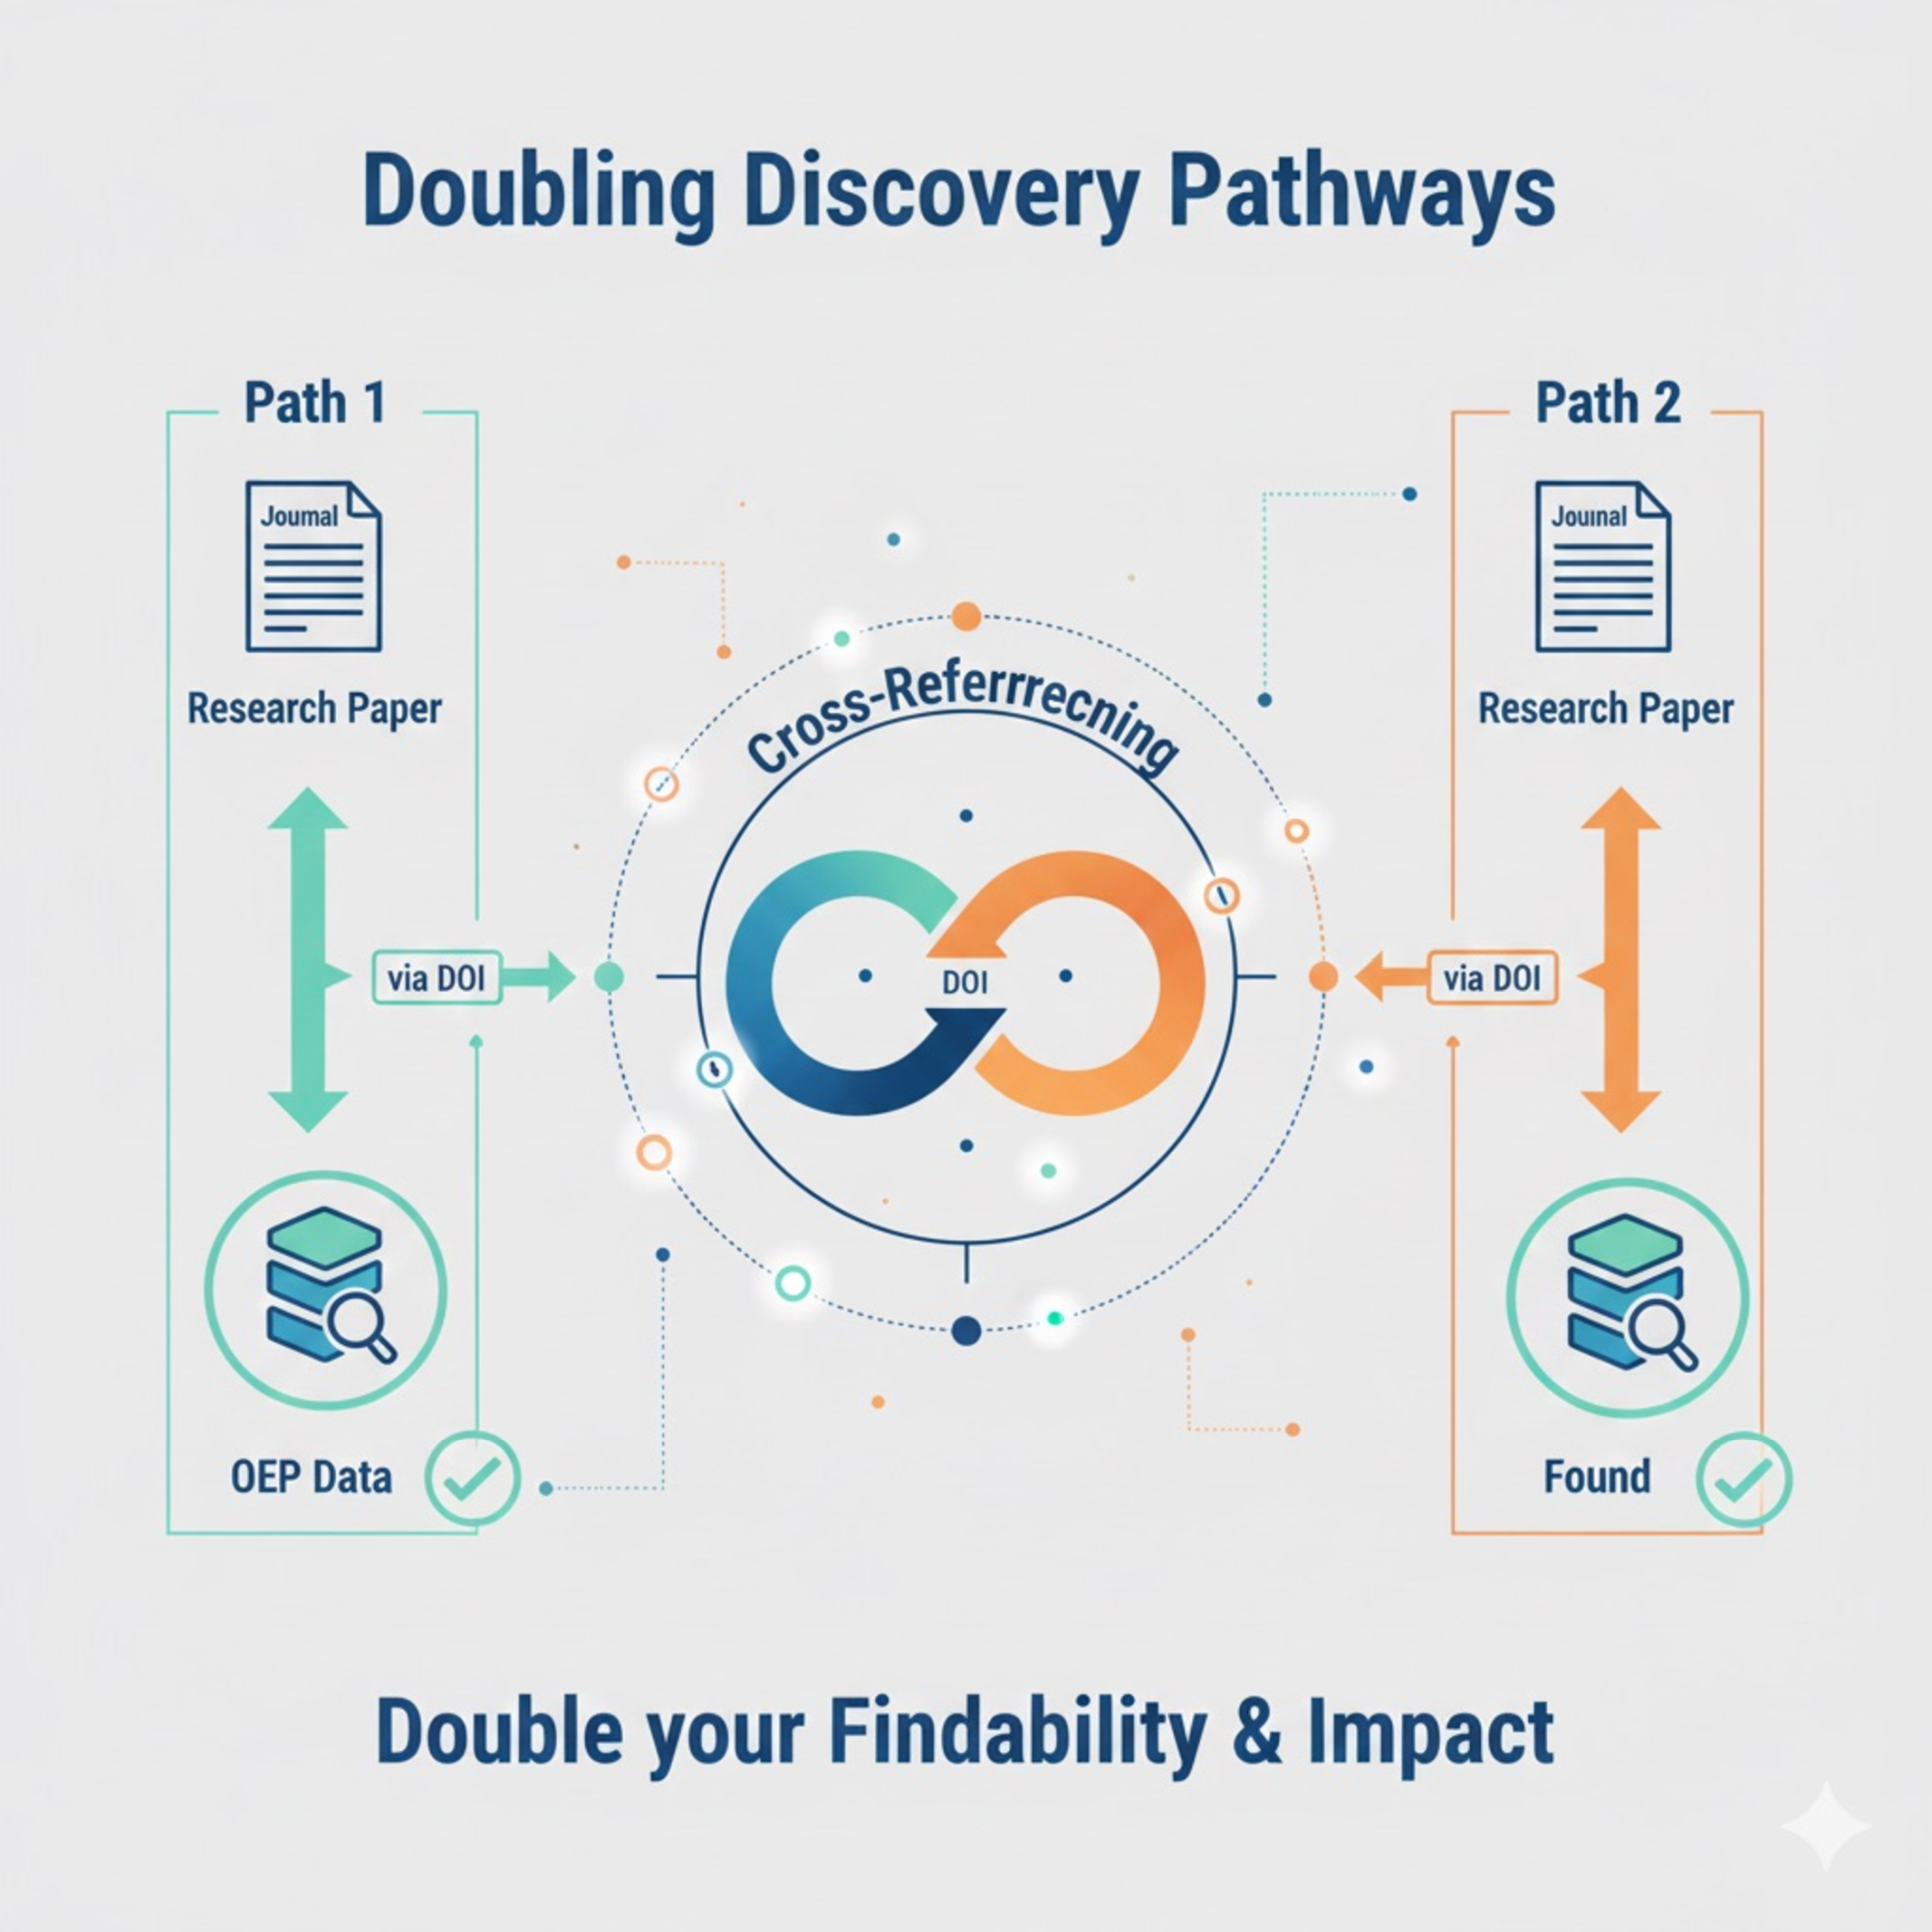
\includegraphics[width=.8\textwidth]{figs/fig_d2p6/fig_d2p6_04-paths}
        \end{center}
        
        \column{.74\textwidth}
        \textbf{Justification:} Why link your OEP data to your journal paper?
        \pause
        
        \begin{itemize}
            \item \textbf{Path 1:} Researcher finds your \textbf{Paper}. The paper links to the \textbf{OEP} data (via DOI). $\rightarrow$ \textbf{Data is Found!}
            \pause
            \item \textbf{Path 2:} Researcher finds your \textbf{OEP Data}. The metadata links to the \textbf{Paper} (via DOI). $\rightarrow$ \textbf{Paper is Found!}
        \end{itemize}
        
        \pause
        
        By \textbf{cross-referencing}, you double the pathways to your work, dramatically increasing its \textbf{Findability} and potential \textbf{Impact}.
        
    \end{columns}
    
\end{frame}

\begin{frame}{Interactive: Appraise and Justify}{Module 6.5: Practice}
    \begin{block}{Discussion (10 min)}
        \textbf{Task 1: Appraise}
        \begin{itemize}
            \item Your colleague wants to use a `CC-BY-ND` (No-Derivatives) license "so nobody can misrepresent my data." \textbf{Appraise} this choice. Is it good for FAIR?
        \end{itemize}
        \pause
        \textbf{Task 2: Justify}
        \begin{itemize}
            \item \textbf{Justify} (in one sentence) why you must include your ORCID iD in your KITOpen submission. (Hint: It links your \textit{data} to your \textit{person}).
        \end{itemize}
    \end{block}
\end{frame}

\begin{frame}{Learning Objectives (6.6)}
    \begin{itemize}
        \item \textbf{Draft} the final, publicly visible \textbf{data citation} and \textbf{abstract} for a dataset, optimising for findability.
        \item \textbf{Synthesize} a final publication strategy that integrates \textbf{KITOpen} and \textbf{OEP}.
    \end{itemize}
\end{frame}

\begin{frame}{Theory: Writing a "Data Abstract"}{Module 6.6: Draft}
    Your Data Abstract is \textbf{not} your Paper Abstract. It's "SEO" for your data.
    
    \begin{columns}
        \column{.4\textwidth}
        \begin{block}{Bad Data Abstract}
            "This file contains the data for our recent paper. See the paper for details."
        \end{block}
        \vspace{3.2ex}
        \pause
        \textbf{Problem:} No keywords. No context. Not findable.
        
        \column{.6\textwidth}
        \begin{block}{Good Data Abstract}
            "This dataset contains raw data from a 2025 simulation of the German power grid, focusing on the NUTS-3 region of Karlsruhe (DE122). Data includes hourly load profiles and wind generation, modelled using [Software]... "
        \end{block}
        \pause
            \textbf{Result:} Rich with keywords. Highly findable.
    \end{columns}
\end{frame}

\begin{frame}{Theory: The "Both" Strategy}{Module 6.6: Synthesise}
    You don't have to choose between KITOpen and OEP. The best strategy is to use \textbf{both}.
    
    \begin{block}{The "HMC/KIT" Best Practice Strategy}
        \begin{enumerate}
            \item \textbf{Archive (Integrity):} Deposit the full, final, static dataset on \textbf{KITOpen}. This fulfils your institutional duty and gets a permanent DOI for long-term archiving.
            \pause
            \item \textbf{Index (Interoperability):} Create a \emph{new metadata record} on \textbf{OEP}.
            \pause
            \item \textbf{Link (Findability):} In the OEP record, do \textbf{not} re-upload the data. Instead, point to the \textbf{KITOpen DOI}.
        \end{enumerate}
    \end{block}
    \pause
    \textbf{Result:} You get the long-term integrity of KITOpen \emph{and} the domain-specific findability of OEP.
\end{frame}

\begin{frame}{Interactive: Your Final Strategy}{Module 6.6: Practice}
    \begin{block}{Final Activity (15 min)}
        \textbf{Task 1: Draft}
        \begin{itemize}
            \item Take 5 minutes and \textbf{draft} a "good" data abstract (2-3 sentences) for your own research data. Focus on keywords.
        \end{itemize}
        \pause
        \textbf{Task 2: Synthesise}
        \begin{itemize}
            \item \textbf{Synthesize} your final publication strategy. How will you use both your institutional and domain repositories?
            \item Share your plan.
        \end{itemize}
    \end{block}
\end{frame}

\begin{frame}{Workshop Summary}
    \begin{columns}
        \column{.5\textwidth}
        \begin{block}{Day 1: Foundations}
            \begin{itemize}
                \item Integrity $\rightarrow$ FAIR
                \item DMP $\rightarrow$ RDMO
                \item Operations $\rightarrow$ ELN, Git, Pipelines
            \end{itemize}
        \end{block}
        
        \column{.5\textwidth}
        \begin{block}{Day 2: Metadata}
            \begin{itemize}
                \item Serialisation (XML, JSON)
                \item Semantics (CV, Ontology)
                \item Publishing (KITOpen, OEP)
            \end{itemize}
        \end{block}
    \end{columns}
    \vfill
    \begin{block}{All Goals Achieved!}
        You can now connect Data Integrity to FAIR, build a DMP in RDMO, integrate RDM into operations, serialise and semantically enrich metadata, and publish on KITOpen and OEP.
    \end{block}
\end{frame}

\begin{frame}{Thank You}
    \begin{center}
        \vfill
        \Huge{\textbf{Questions?}}
        \vfill
        \vfill
        \large{Helmholtz Metadata Collaboration (HMC)} \\
        \large{Karlsruhe Institute of Technology (KIT)}
    \end{center}
\end{frame}